%%%%%%%%%%%%%%%%%%%%%%%%%%%%%%%%%%%%%%%%%
%  My documentation report
%  Objetive: Explain what I did and how, so someone can continue with the investigation
%
% Important note:
% Chapter heading images should have a 2:1 width:height ratio,
% e.g. 920px width and 460px height.
%
%%%%%%%%%%%%%%%%%%%%%%%%%%%%%%%%%%%%%%%%%


%----------------------------------------------------------------------------------------
%	PACKAGES AND OTHER DOCUMENT CONFIGURATIONS
%----------------------------------------------------------------------------------------

\documentclass[11pt,fleqn]{book} % Default font size and left-justified equations

\usepackage[top=3cm,bottom=3cm,left=3.2cm,right=3.2cm,headsep=10pt,letterpaper]{geometry} % Page margins

\usepackage{xcolor} % Required for specifying colors by name
\definecolor{ocre}{RGB}{52,177,201} % Define the orange color used for highlighting throughout the book

% Font Settings
\usepackage{avant} % Use the Avantgarde font for headings
%\usepackage{times} % Use the Times font for headings
\usepackage{mathptmx} % Use the Adobe Times Roman as the default text font together with math symbols from the Sym­bol, Chancery and Com­puter Modern fonts
\usepackage{microtype} % Slightly tweak font spacing for aesthetics
\usepackage[utf8]{inputenc} % Required for including letters with accents
\usepackage[T1]{fontenc} % Use 8-bit encoding that has 256 glyphs
\usepackage{amsthm}

\usepackage{multicol}
\usepackage{caption}
\usepackage{graphicx}
\usepackage{subcaption}
\usepackage{dirtytalk}
\usepackage[autostyle=true]{csquotes}

\usepackage[framemethod=tikz]{mdframed}
\usepackage{environ}
\usepackage{lipsum}

% Bibliography
\usepackage[style=alphabetic,sorting=nyt,sortcites=true,autopunct=true,babel=hyphen,hyperref=true,abbreviate=false,backref=true,backend=biber]{biblatex}
\addbibresource{bibliography.bib} % BibTeX bibliography file
\defbibheading{bibempty}{}

%----------------------------------------------------------------------------------------
%	VARIOUS REQUIRED PACKAGES
%----------------------------------------------------------------------------------------

\usepackage{titlesec} % Allows customization of titles

\usepackage{graphicx} % Required for including pictures
\graphicspath{{Pictures/}} % Specifies the directory where pictures are stored
% \graphicspath{{Plots/}}
\usepackage{lipsum} % Inserts dummy text

\usepackage{tikz} % Required for drawing custom shapes

\usepackage[english]{babel} % English language/hyphenation

\usepackage{enumitem} % Customize lists
\setlist{nolistsep} % Reduce spacing between bullet points and numbered lists

\usepackage{booktabs} % Required for nicer horizontal rules in tables

\usepackage{eso-pic} % Required for specifying an image background in the title page

%----------------------------------------------------------------------------------------
%	MAIN TABLE OF CONTENTS
%----------------------------------------------------------------------------------------

\usepackage{titletoc} % Required for manipulating the table of contents

\contentsmargin{0cm} % Removes the default margin
% Chapter text styling
\titlecontents{chapter}[1.25cm] % Indentation
{\addvspace{15pt}\large\sffamily\bfseries} % Spacing and font options for chapters
{\color{ocre!60}\contentslabel[\Large\thecontentslabel]{1.25cm}\color{ocre}} % Chapter number
{}
{\color{ocre!60}\normalsize\sffamily\bfseries\;\titlerule*[.5pc]{.}\;\thecontentspage} % Page number
% Section text styling
\titlecontents{section}[1.25cm] % Indentation
{\addvspace{5pt}\sffamily\bfseries} % Spacing and font options for sections
{\contentslabel[\thecontentslabel]{1.25cm}} % Section number
{}
{\sffamily\hfill\color{black}\thecontentspage} % Page number
[]
% Subsection text styling
\titlecontents{subsection}[1.25cm] % Indentation
{\addvspace{1pt}\sffamily\small} % Spacing and font options for subsections
{\contentslabel[\thecontentslabel]{1.25cm}} % Subsection number
{}
{\sffamily\;\titlerule*[.5pc]{.}\;\thecontentspage} % Page number
[]

%----------------------------------------------------------------------------------------
%	MINI TABLE OF CONTENTS IN CHAPTER HEADS
%----------------------------------------------------------------------------------------

% Section text styling
\titlecontents{lsection}[0em] % Indendating
{\footnotesize\sffamily} % Font settings
{}
{}
{}

% Subsection text styling
\titlecontents{lsubsection}[.5em] % Indentation
{\normalfont\footnotesize\sffamily} % Font settings
{}
{}
{}

%----------------------------------------------------------------------------------------
%	PAGE HEADERS
%----------------------------------------------------------------------------------------

\usepackage{fancyhdr} % Required for header and footer configuration

\pagestyle{fancy}
\renewcommand{\chaptermark}[1]{\markboth{\sffamily\normalsize\bfseries\chaptername\ \thechapter.\ #1}{}} % Chapter text font settings
\renewcommand{\sectionmark}[1]{\markright{\sffamily\normalsize\thesection\hspace{5pt}#1}{}} % Section text font settings
\fancyhf{} \fancyhead[LE,RO]{\sffamily\normalsize\thepage} % Font setting for the page number in the header
\fancyhead[LO]{\rightmark} % Print the nearest section name on the left side of odd pages
\fancyhead[RE]{\leftmark} % Print the current chapter name on the right side of even pages
\renewcommand{\headrulewidth}{0.5pt} % Width of the rule under the header
\addtolength{\headheight}{2.5pt} % Increase the spacing around the header slightly
\renewcommand{\footrulewidth}{0pt} % Removes the rule in the footer
\fancypagestyle{plain}{\fancyhead{}\renewcommand{\headrulewidth}{0pt}} % Style for when a plain pagestyle is specified

% Removes the header from odd empty pages at the end of chapters
\makeatletter
\renewcommand{\cleardoublepage}{
\clearpage\ifodd\c@page\else
\hbox{}
\vspace*{\fill}
\thispagestyle{empty}
\newpage
\fi}

%----------------------------------------------------------------------------------------
%	THEOREM STYLES
%----------------------------------------------------------------------------------------

\usepackage{amsmath,amsfonts,amssymb,amsthm} % For math equations, theorems, symbols, etc

\newcommand{\intoo}[2]{\mathopen{]}#1\,;#2\mathclose{[}}
\newcommand{\ud}{\mathop{\mathrm{{}d}}\mathopen{}}
\newcommand{\intff}[2]{\mathopen{[}#1\,;#2\mathclose{]}}
\newtheorem{notation}{Notation}[chapter]

%%%%%%%%%%%%%%%%%%%%%%%%%%%%%%%%%%%%%%%%%%%%%%%%%%%%%%%%%%%%%%%%%%%%%%%%%%%
%%%%%%%%%%%%%%%%%%%% dedicated to boxed/framed environements %%%%%%%%%%%%%%
%%%%%%%%%%%%%%%%%%%%%%%%%%%%%%%%%%%%%%%%%%%%%%%%%%%%%%%%%%%%%%%%%%%%%%%%%%%
\newtheoremstyle{ocrenumbox}% % Theorem style name
{0pt}% Space above
{0pt}% Space below
{\normalfont}% % Body font
{}% Indent amount
{\small\bf\sffamily\color{ocre}}% % Theorem head font
{\;}% Punctuation after theorem head
{0.25em}% Space after theorem head
{\small\sffamily\color{ocre}\thmname{#1}\nobreakspace\thmnumber{\@ifnotempty{#1}{}\@upn{#2}}% Theorem text (e.g. Theorem 2.1)
\thmnote{\nobreakspace\the\thm@notefont\sffamily\bfseries\color{black}---\nobreakspace#3.}} % Optional theorem note
\renewcommand{\qedsymbol}{$\blacksquare$}% Optional qed square

\newtheoremstyle{blacknumex}% Theorem style name
{5pt}% Space above
{5pt}% Space below
{\normalfont}% Body font
{} % Indent amount
{\small\bf\sffamily}% Theorem head font
{\;}% Punctuation after theorem head
{0.25em}% Space after theorem head
{\small\sffamily{\tiny\ensuremath{\blacksquare}}\nobreakspace\thmname{#1}\nobreakspace\thmnumber{\@ifnotempty{#1}{}\@upn{#2}}% Theorem text (e.g. Theorem 2.1)
\thmnote{\nobreakspace\the\thm@notefont\sffamily\bfseries---\nobreakspace#3.}}% Optional theorem note

\newtheoremstyle{blacknumbox} % Theorem style name
{0pt}% Space above
{0pt}% Space below
{\normalfont}% Body font
{}% Indent amount
{\small\bf\sffamily}% Theorem head font
{\;}% Punctuation after theorem head
{0.25em}% Space after theorem head
{\small\sffamily\thmname{#1}\nobreakspace\thmnumber{\@ifnotempty{#1}{}\@upn{#2}}% Theorem text (e.g. Theorem 2.1)
\thmnote{\nobreakspace\the\thm@notefont\sffamily\bfseries---\nobreakspace#3.}}% Optional theorem note

%%%%%%%%%%%%%%%%%%%%%%%%%%%%%%%%%%%%%%%%%%%%%%%%%%%%%%%%%%%%%%%%%%%%%%%%%%%
%%%%%%%%%%%%% dedicated to non-boxed/non-framed environements %%%%%%%%%%%%%
%%%%%%%%%%%%%%%%%%%%%%%%%%%%%%%%%%%%%%%%%%%%%%%%%%%%%%%%%%%%%%%%%%%%%%%%%%%
\newtheoremstyle{ocrenum}% % Theorem style name
{5pt}% Space above
{5pt}% Space below
{\normalfont}% % Body font
{}% Indent amount
{\small\bf\sffamily\color{ocre}}% % Theorem head font
{\;}% Punctuation after theorem head
{0.25em}% Space after theorem head
{\small\sffamily\color{ocre}\thmname{#1}\nobreakspace\thmnumber{\@ifnotempty{#1}{}\@upn{#2}}% Theorem text (e.g. Theorem 2.1)
\thmnote{\nobreakspace\the\thm@notefont\sffamily\bfseries\color{black}---\nobreakspace#3.}} % Optional theorem note
\renewcommand{\qedsymbol}{$\blacksquare$}% Optional qed square
\makeatother

% Defines the theorem text style for each type of theorem to one of the three styles above
\newcounter{dummy}
\numberwithin{dummy}{section}
\theoremstyle{ocrenumbox}


\newtheorem{theoremeT}[dummy]{Theorem}
\newtheorem{lemma}[dummy]{Lemma}
\newtheorem{observation}[dummy]{Observation}
\newtheorem{proposition}[dummy]{Proposition}
% \newtheorem{definition}[dummy]{Definition}
\newtheorem{claim}[dummy]{Claim}
\newtheorem{fact}[dummy]{Fact}
\newtheorem{assumption}[dummy]{Assumption}

\newtheorem{problem}{Problem}[chapter]
% \newtheorem{exercise}{Exercise}[chapter]
\theoremstyle{blacknumex}
\newtheorem{exampleT}{Example}[chapter]
\theoremstyle{blacknumbox}
\newtheorem{vocabulary}{Vocabulary}[chapter]
\newtheorem{definitionT}{Definition}[section]
\newtheorem{corollaryT}[dummy]{Corollary}
\theoremstyle{ocrenum}

%----------------------------------------------------------------------------------------
%	DEFINITION OF COLORED BOXES
%----------------------------------------------------------------------------------------

\RequirePackage[framemethod=default]{mdframed} % Required for creating the theorem, definition, exercise and corollary boxes

% Theorem box
\newmdenv[skipabove=7pt,
skipbelow=7pt,
backgroundcolor=black!5,
linecolor=ocre,
innerleftmargin=5pt,
innerrightmargin=5pt,
innertopmargin=5pt,
leftmargin=0cm,
rightmargin=0cm,
innerbottommargin=5pt]{tBox}

% Exercise box
\newmdenv[skipabove=7pt,
skipbelow=7pt,
rightline=false,
leftline=true,
topline=false,
bottomline=false,
backgroundcolor=ocre!10,
linecolor=ocre,
innerleftmargin=5pt,
innerrightmargin=5pt,
innertopmargin=5pt,
innerbottommargin=5pt,
leftmargin=0cm,
rightmargin=0cm,
linewidth=4pt]{eBox}

% Definition box
\newmdenv[skipabove=7pt,
skipbelow=7pt,
rightline=false,
leftline=true,
topline=false,
bottomline=false,
linecolor=ocre,
innerleftmargin=5pt,
innerrightmargin=5pt,
innertopmargin=0pt,
leftmargin=0cm,
rightmargin=0cm,
linewidth=4pt,
innerbottommargin=0pt]{dBox}

% Corollary box
\newmdenv[skipabove=7pt,
skipbelow=7pt,
rightline=false,
leftline=true,
topline=false,
bottomline=false,
linecolor=gray,
backgroundcolor=black!5,
innerleftmargin=5pt,
innerrightmargin=5pt,
innertopmargin=5pt,
leftmargin=0cm,
rightmargin=0cm,
linewidth=4pt,
innerbottommargin=5pt]{cBox}

% Creates an environment for each type of theorem and assigns it a theorem text style from the "Theorem Styles" section above and a colored box from above
\newenvironment{theorem}{\begin{tBox}\begin{theoremeT}}{\end{theoremeT}\end{tBox}}
\newenvironment{exercise}{\begin{eBox}\begin{exerciseT}}{\hfill{\color{ocre}\tiny\ensuremath{\blacksquare}}\end{exerciseT}\end{eBox}}
\newenvironment{definition}{\begin{dBox}\begin{definitionT}}{\end{definitionT}\end{dBox}}
\newenvironment{example}{\begin{exampleT}}{\hfill{\tiny\ensuremath{\blacksquare}}\end{exampleT}}
\newenvironment{corollary}{\begin{cBox}\begin{corollaryT}}{\end{corollaryT}\end{cBox}}

%----------------------------------------------------------------------------------------
%	REMARK ENVIRONMENT
%----------------------------------------------------------------------------------------

\newenvironment{remark}{\par\vspace{10pt}\small % Vertical white space above the remark and smaller font size
\begin{list}{}{
\leftmargin=35pt % Indentation on the left
\rightmargin=25pt}\item\ignorespaces % Indentation on the right
\makebox[-2.5pt]{\begin{tikzpicture}[overlay]
\node[draw=ocre!60,line width=1pt,circle,fill=ocre!25,font=\sffamily\bfseries,inner sep=2pt,outer sep=0pt] at (-15pt,0pt){\textcolor{ocre}{R}};\end{tikzpicture}} % Orange R in a circle
\advance\baselineskip -1pt}{\end{list}\vskip5pt} % Tighter line spacing and white space after remark

%----------------------------------------------------------------------------------------
%	SECTION NUMBERING IN THE MARGIN
%----------------------------------------------------------------------------------------

\makeatletter
\renewcommand{\@seccntformat}[1]{\llap{\textcolor{ocre}{\csname the#1\endcsname}\hspace{1em}}}
\renewcommand{\section}{\@startsection{section}{1}{\z@}
{-4ex \@plus -1ex \@minus -.4ex}
{1ex \@plus.2ex }
{\normalfont\large\sffamily\bfseries}}
\renewcommand{\subsection}{\@startsection {subsection}{2}{\z@}
{-3ex \@plus -0.1ex \@minus -.4ex}
{0.5ex \@plus.2ex }
{\normalfont\sffamily\bfseries}}
\renewcommand{\subsubsection}{\@startsection {subsubsection}{3}{\z@}
{-2ex \@plus -0.1ex \@minus -.2ex}
{.2ex \@plus.2ex }
{\normalfont\small\sffamily\bfseries}}
\renewcommand\paragraph{\@startsection{paragraph}{4}{\z@}
{-2ex \@plus-.2ex \@minus .2ex}
{.1ex}
{\normalfont\small\sffamily\bfseries}}

%----------------------------------------------------------------------------------------
%	HYPERLINKS IN THE DOCUMENTS
%----------------------------------------------------------------------------------------

% For an unclear reason, the package should be loaded now and not later
\usepackage{hyperref}
\hypersetup{hidelinks,backref=true,pagebackref=true,hyperindex=true,colorlinks=false,breaklinks=true,urlcolor= ocre,bookmarks=true,bookmarksopen=false,pdftitle={Title},pdfauthor={Author}}

%----------------------------------------------------------------------------------------
%	CHAPTER HEADINGS
%----------------------------------------------------------------------------------------

% The set-up below should be (sadly) manually adapted to the overall margin page septup controlled by the geometry package loaded in the main.tex document. It is possible to implement below the dimensions used in the goemetry package (top,bottom,left,right)... TO BE DONE

\newcommand{\thechapterimage}{}
\newcommand{\chapterimage}[1]{\renewcommand{\thechapterimage}{#1}}

% Numbered chapters with mini tableofcontents
\def\thechapter{\arabic{chapter}}
\def\@makechapterhead#1{
\thispagestyle{empty}
{\centering \normalfont\sffamily
\ifnum \c@secnumdepth >\m@ne
\if@mainmatter
\startcontents
\begin{tikzpicture}[remember picture,overlay]
\node at (current page.north west)
{\begin{tikzpicture}[remember picture,overlay]
\node[anchor=north west,inner sep=0pt] at (0,0) {\includegraphics[width=\paperwidth]{\thechapterimage}};
%%%%%%%%%%%%%%%%%%%%%%%%%%%%%%%%%%%%%%%%%%%%%%%%%%%%%%%%%%%%%%%%%%%%%%%%%%%%%%%%%%%%%
% Commenting the 3 lines below removes the small contents box in the chapter heading
%\fill[color=ocre!10!white,opacity=.6] (1cm,0) rectangle (8cm,-7cm);
%\node[anchor=north west] at (1.1cm,.35cm) {\parbox[t][8cm][t]{6.5cm}{\huge\bfseries\flushleft \printcontents{l}{1}{\setcounter{tocdepth}{2}}}};
\draw[anchor=west] (5cm,-9cm) node [rounded corners=20pt,fill=ocre!10!white,text opacity=1,draw=ocre,draw opacity=1,line width=1.5pt,fill opacity=.6,inner sep=12pt]{\huge\sffamily\bfseries\textcolor{black}{\thechapter. #1\strut\makebox[22cm]{}}};
%%%%%%%%%%%%%%%%%%%%%%%%%%%%%%%%%%%%%%%%%%%%%%%%%%%%%%%%%%%%%%%%%%%%%%%%%%%%%%%%%%%%%
\end{tikzpicture}};
\end{tikzpicture}}
\par\vspace*{230\p@}
\fi
\fi}

% Unnumbered chapters without mini tableofcontents (could be added though)
\def\@makeschapterhead#1{
\thispagestyle{empty}
{\centering \normalfont\sffamily
\ifnum \c@secnumdepth >\m@ne
\if@mainmatter
\begin{tikzpicture}[remember picture,overlay]
\node at (current page.north west)
{\begin{tikzpicture}[remember picture,overlay]
\node[anchor=north west,inner sep=0pt] at (0,0) {\includegraphics[width=\paperwidth]{\thechapterimage}};
\draw[anchor=west] (5cm,-9cm) node [rounded corners=20pt,fill=ocre!10!white,fill opacity=.6,inner sep=12pt,text opacity=1,draw=ocre,draw opacity=1,line width=1.5pt]{\huge\sffamily\bfseries\textcolor{black}{#1\strut\makebox[22cm]{}}};
\end{tikzpicture}};
\end{tikzpicture}}
\par\vspace*{230\p@}
\fi
\fi
}
\makeatother
 % Insert the commands.tex file which contains the majority of the structure behind the template

\SetMainLanguage{english} % or your main language


\newtheorem{question}{Question}
\mdfdefinestyle{que}{
  linecolor=cyan,
  backgroundcolor=cyan!20,
}
\surroundwithmdframed[style=que]{question}

\newtheorem{answer}{Answer}
\mdfdefinestyle{ans}{
  linecolor=cyan,
  backgroundcolor=yellow!20
}
\surroundwithmdframed[style=ans]{answer}

\NewEnviron{rotanswer}{%
  \begin{tikzpicture}
  \node[rotate=180,inner sep=0pt] {\parbox{\linewidth}{%
  \begin{answer}
  \BODY
  \end{answer}}};
\end{tikzpicture}%
}


%----------------------------------------------------------------------------------------
%	Definitions of new commands
%----------------------------------------------------------------------------------------

\def\R{\mathbb{R}}
\newcommand{\cvx}{convex}
\begin{document}

%----------------------------------------------------------------------------------------
%	TITLE PAGE
%----------------------------------------------------------------------------------------

\begingroup
\thispagestyle{empty}
\AddToShipoutPicture*{\put(0,0){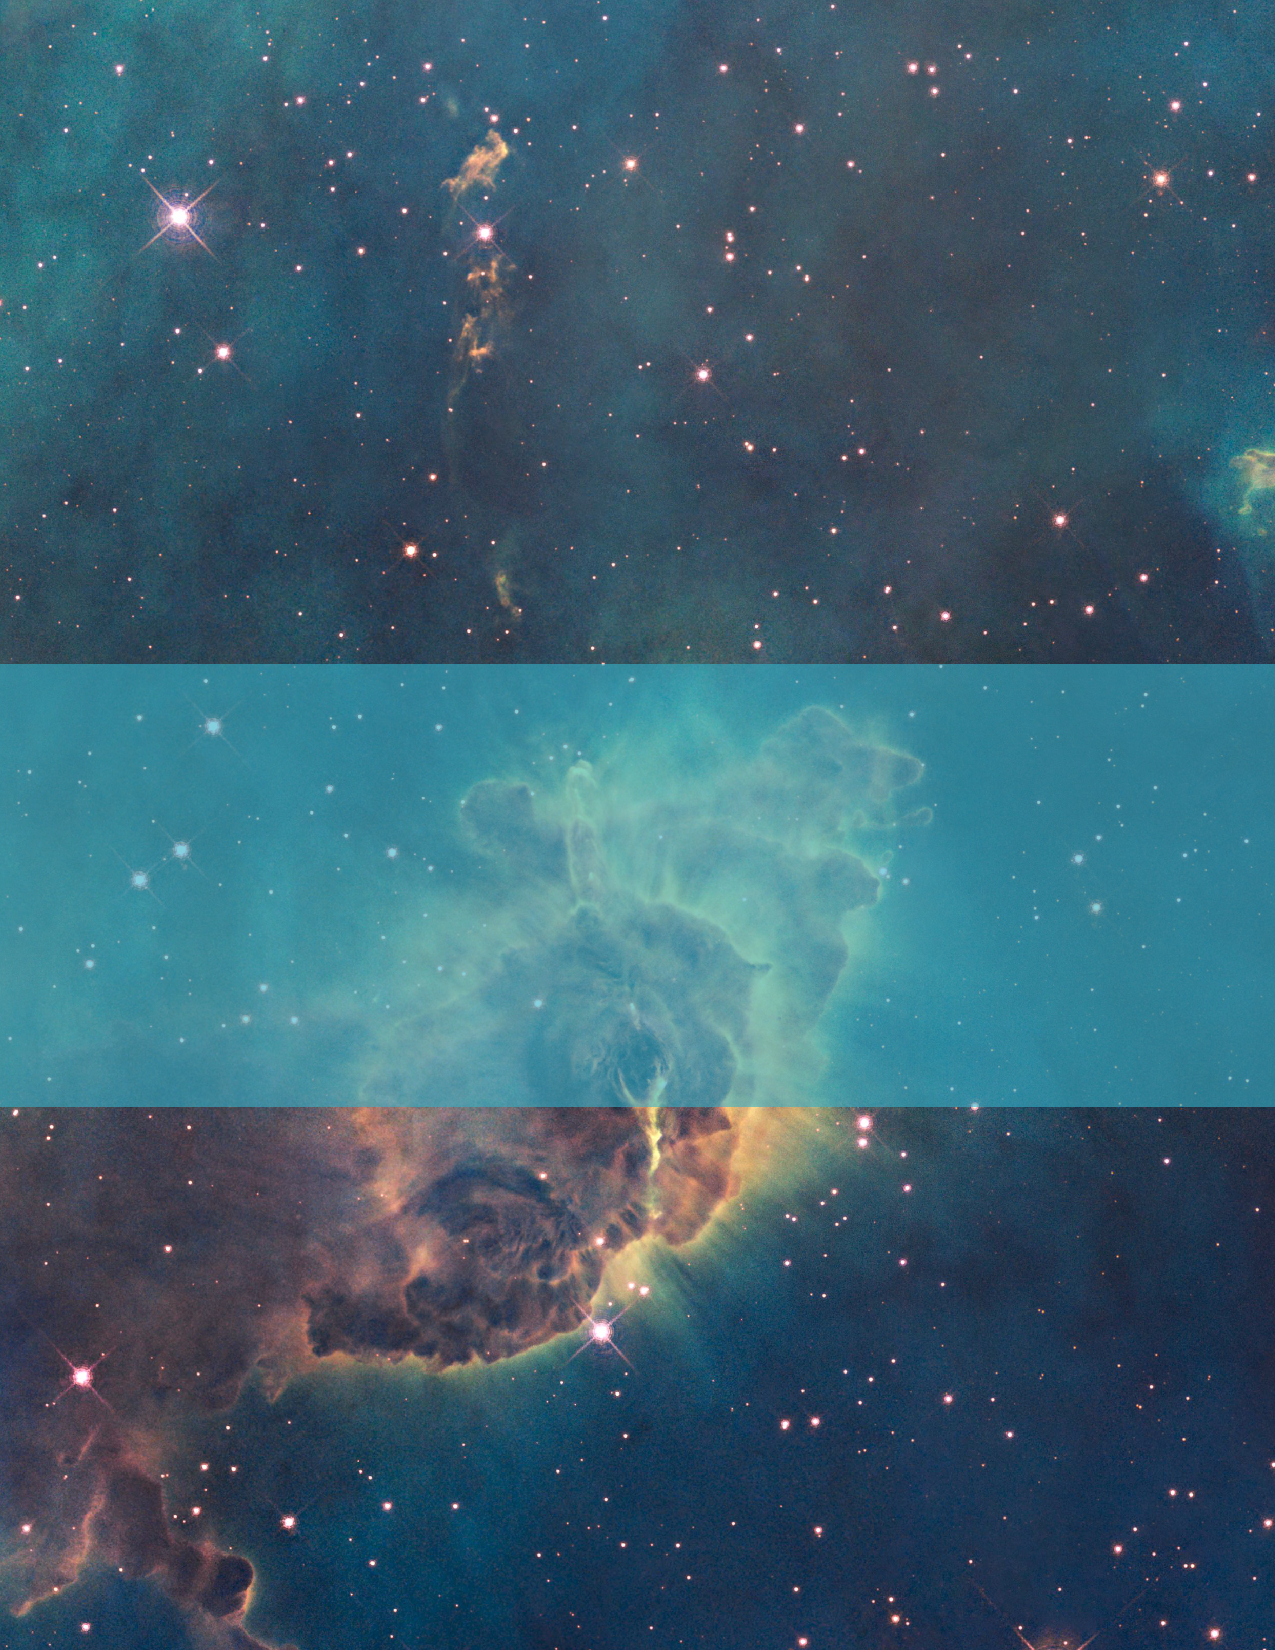
\includegraphics[scale=1.25]{esahubble}}} % Image background
\centering
\vspace*{5cm}
\par\normalfont\fontsize{35}{35}\sffamily\selectfont
\textbf{Business Analytics Notes}\\
{\LARGE BSMS2002 Lecture Notes for Weeks 1 to 12}\par % Book title
\vspace*{1cm}
{\Huge Sayan Ghosh}\par % Author name
\endgroup

%----------------------------------------------------------------------------------------
%	COPYRIGHT PAGE
%----------------------------------------------------------------------------------------

\newpage
~\vfill
\thispagestyle{empty}

%\noindent Copyright \copyright\ 2014 Andrea Hidalgo\\ % Copyright notice

\noindent \textsc{Business Analytics (BSMS2002) Lecture Notes}\\

\noindent \textsc{\url{https://github.com/sayan01/ba-notes}}\\ % URL

\noindent This document contains my personal lecture notes
of the Business Analytics (BSMS2002) course taught by
\textbf{
\href{https://doms.iitm.ac.in/index.php/rrm}{Prof. Rahul Marathe R.}
}
at
\textbf{
\href{https://study.iitm.ac.in/ds/}{IIT Madras BS Program}.
}
This is not an official document.\\ % License information

\noindent \textit{First release, January 2024} % Printing/edition date

%----------------------------------------------------------------------------------------
%	TABLE OF CONTENTS
%----------------------------------------------------------------------------------------

\chapterimage{head1.png} % Table of contents heading image

\pagestyle{empty} % No headers

\tableofcontents % Print the table of contents itself

%\cleardoublepage % Forces the first chapter to start on an odd page so it's on the right

\pagestyle{fancy} % Print headers again

%----------------------------------------------------------------------------------------
%	CHAPTER 1
%----------------------------------------------------------------------------------------

\chapterimage{head2.png} % Chapter heading image
\chapter{Week 1: Why Visualize Data?}
\section{Introduction to Data Visualization}
Good data visualization is the key to communicate information clearly and efficiently to users. It is a key step to understand data and make better business decisions.\\
\subsection{Types of Data}
There are broadly two types of data:
\begin{itemize}
\item \textbf{Qualitative or Categorical Data:} Qualitative data is descriptive information \\
\textbf{Examples:} Colors, textures, smells, tastes, appearance, beauty, etc.
\item \textbf{Quantitative or Numeric Data:} Quantitative data is numerical information (numbers)\\
\textbf{Examples:} Counts, height, weight, area, volume, ratings, etc.
\end{itemize}
\subsection{Categorical Data}
\begin{definition}[Categorical Data]
Categorical data is a type of data that is used to group information with similar characteristics.
\end{definition}
Categorical data are labels and the values can belong to only
a specific set of categories.\\

They can be further divided into two types:
\begin{itemize}
\item \textbf{Nominal Data:} Nominal data is a type of data that is used to label variables without providing any quantitative value or ordering.\\
\item \textbf{Ordinal Data:} Ordinal data is a type of data that is used to label variables, but the order of the values matters.\\
\end{itemize}

\newpage

\subsection{Numeric Data}
\begin{definition}[Numeric Data Data]
Quantitative or Numeric data is a type of data that is used to measure things.
\end{definition}
It can either be
\textbf{discrete} or \textbf{continuous}.

\begin{definition}[Discrete Data]
Discrete data is a type of data that can only take certain values.\\
\end{definition}

\begin{definition}[Continuous Data]
Continuous data is a type of data that can take any value.\\
\end{definition}

\begin{example}
  The height of a person is a continuous numeric variable.
\end{example}
\begin{example}
  The number of students in a class is a discrete numeric variable.
\end{example}
\begin{example}
  The gender of a person is a categorical variable.
\end{example}


\subsubsection{Benefits of Visualizing Data}
\begin{itemize}
    \item \textbf{Communicate complex information:}
      Visualizations help people understand data quickly
      and convey a lot of information concisely and powerfully.
    \item \textbf{A Picture is worth a thousand words:}
      Create a “picture” for reasoning about and analyzing
      quantitative and conceptual information.
      \begin{itemize}
        \item Makes cognitive processing easier
        \item Provides “content/information rich” view at a glance
        \item Directs attention toward the content rather than methodology
      \end{itemize}
    \item \textbf{Focus on the important:}
      % Convey a message about the significance of the data
      Visualizations help you focus on the important parts of the data
      and give you a clear idea of what the data is trying to tell you.
      It lets us identify which factors are more significant than others.
\end{itemize}

\subsubsection{Attributes of Visual Perception}
\begin{multicols}{2}
\begin{itemize}
  \item \textbf{Form:}
    \begin{itemize}
      \item Length
      \item Width
      \item Orientation
      \item Size
      \item Shape
      \item Curvature
      \item Enclosure
      \item Spatial grouping
      \item Blur
    \end{itemize}
  \item \textbf{Color:}
    \begin{itemize}
      \item Hue
      \item Saturation
      \item Brightness
    \end{itemize}
  \item \textbf{Position:}
    \begin{itemize}
      \item 1D: Position along a common scale
      \item 2D: Position in a plane
      \item 3D: Position in space
      \item Direction of motion
    \end{itemize}
\end{itemize}
\end{multicols}

\begin{figure}[htb!]
    \centering
    \begin{subfigure}[c]{0.45\linewidth}
        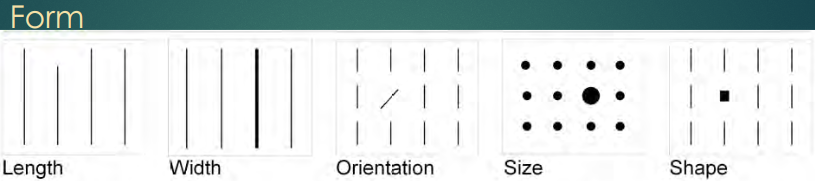
\includegraphics[width=\linewidth]{Pictures/visual-perception-form1.png}
        \label{fig:form1}
    \end{subfigure}
    \begin{subfigure}[c]{0.45\linewidth}
        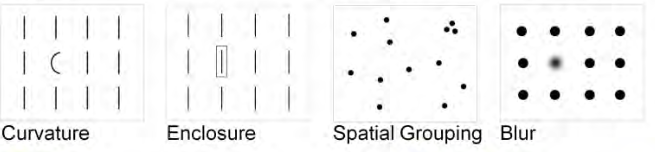
\includegraphics[width=\linewidth]{Pictures/visual-perception-form2.png}
        \label{fig:form2}
    \end{subfigure}
    \caption{Visual Perception: Form}
    \label{fig:visual-perception-form}
\end{figure}



\begin{figure}[htb!]
    \centering
    \begin{subfigure}[c]{0.45\linewidth}
        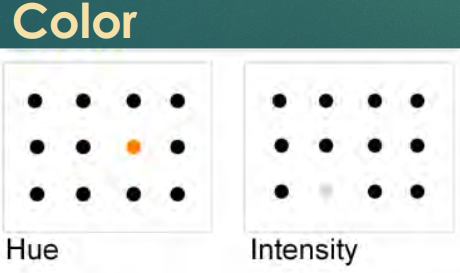
\includegraphics[width=\linewidth]{Pictures/visual-perception-color.png}
        \caption{Visual Perception: Color}
        \label{fig:color}
    \end{subfigure}
    \hfill
    \begin{subfigure}[c]{0.45\linewidth}
        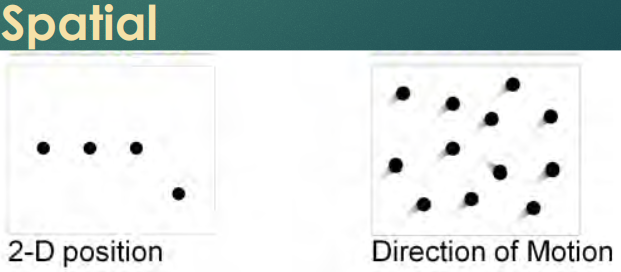
\includegraphics[width=\linewidth]{Pictures/visual-perception-spatial.png}
        \caption{Visual Perception: Spatial}
        \label{fig:spatial}
    \end{subfigure}
    \caption{Visual Perception: Color and Spatial}
    \label{fig:visual-perception-color-spatial}
\end{figure}



\begin{theorem}[Umbrella Principle]
  There are four principles of data visualization:
  \begin{itemize}
    \item \textbf{Know Purpose}: You need to have a purpose
      statement for every visualization you create. A purpose
      is not necessarily a message.
    \item \textbf{Ensure Integrity}: You need to ensure that
      your visualization is accurate and honest. Not just the
      data, but also the visualization itself. The presentation
      should not distort the truth or mislead the audience.
    \item \textbf{Maximize Data Ink; Minimize Non-Data Ink}:
      Make sure unnecessary elements are removed from the
      visualization. The goal is to maximize the data-ink ratio.
    \item \textbf{Show Your Data; Annotate}:
      You need to show your data. You should also annotate
      your visualization to help the audience understand it.
  \end{itemize}
\end{theorem}

\begin{example}
  \textbf{Know Purpose:}
  \say{My purpose in creating this graph
  to help the audience see that only a small
  percentage the patient base are candidates
  for this specific therapeutic regimen.}
\end{example}

\begin{example}
  \textbf{Ensure Integrity:}
  Truncating the y-axis is a common way to
  mislead the audience. The truncated graph
  makes the difference between the two
  groups look much larger than it actually is.
  \begin{figure}[hibt!]
    \centering
    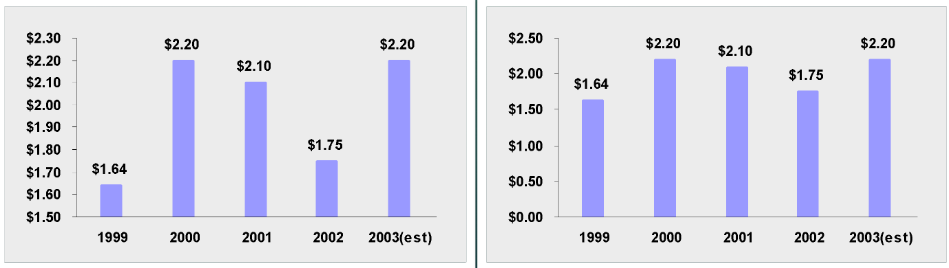
\includegraphics[width=0.8\linewidth]{Pictures/integrity-baseline.png}
    \caption{Baseline Tampering}
    \label{fig:bias-baseline}
  \end{figure}
\end{example}

\begin{example}
  \textbf{Maximize Data Ink; Minimize Non-Data Ink:}
  The graph should only have lines and labels that are
  necessary to understand the data. The graph should
  not have any unnecessary elements like grid lines,
  unnecessary labels, etc.


  \begin{figure}[hitb!]
    \centering
    \begin{subfigure}[c]{0.45\linewidth}
        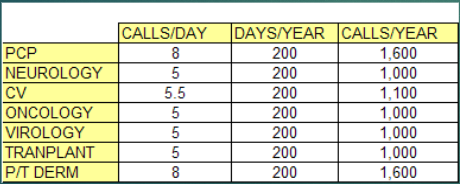
\includegraphics[width=\linewidth]{Pictures/max-data1.png}
        \caption{Cluttered}
        \label{fig:max-data-cluttered}
    \end{subfigure}
    \hfill
    \begin{subfigure}[c]{0.45\linewidth}
        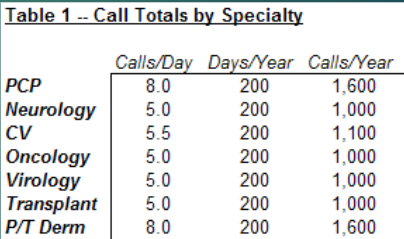
\includegraphics[width=\linewidth]{Pictures/max-data2.png}
        \caption{Clean}
        \label{fig:max-data-clean}
    \end{subfigure}
    \caption{Maximize Data Ink; Minimize Non-Data Ink}
    \label{fig:max-data}
  \end{figure}

\end{example}

\newpage

\begin{example}
  \textbf{Show Your Data; Annotate:}
  You should always show your data. You should also annotate
  your visualization to help the audience understand it.

  \begin{figure}[htb!]
    \centering
    \begin{subfigure}[c]{0.45\linewidth}
        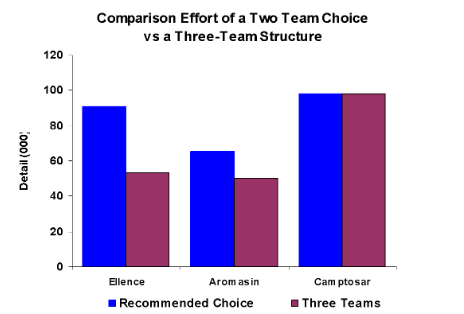
\includegraphics[width=\linewidth]{Pictures/annotate1.png}
        \caption{No Annotations}
        \label{fig:annotate1}
    \end{subfigure}
    \hfill
    \begin{subfigure}[c]{0.45\linewidth}
        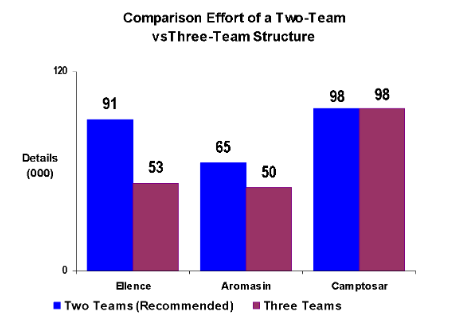
\includegraphics[width=\linewidth]{Pictures/annotate2.png}
        \caption{Annotations}
        \label{fig:annotate2}
    \end{subfigure}
  \end{figure}
\end{example}

\section{Defining the Message}

\begin{definition}[Message]
  The message is the main point that you want to convey to the audience
  through your visualization.
\end{definition}

\subsection{The Three Steps of Data Visualization}

\begin{enumerate}
  \item \textbf{Defining the Message:}
    The first step is to define the message that you want to convey to the audience.
  \item \textbf{Choosing the Right Chart Type:}
    The second step is to choose the right chart type to convey the message.
    \say{Should I use a bar chart or a line chart? or maybe a pie chart?}
  \item \textbf{Designing the Visualization:}
    The third step is to design the visualization.
    \say{What colors should I use? Should I use a 3D chart or a 2D chart?}
    This step should ensure quick cognitive processing of the visualization.
\end{enumerate}

\subsection{One Data, Many Messages}

A single data set can have many messages.
The message that you want to convey
depends on the audience and the context.\\

\begin{example} AIDS Data\\

  You have been given the data of AIDS patients in the US.
  You can use this data to convey many messages:

  \begin{center}
  \begin{tabular}{|c|c|}
    \hline
    \textbf{Age Group} & \textbf{Number of AIDS Cases} \\
    \hline
    Under 5 & 6,975 \\
    5-12 & 2,099 \\
    13-19 & 4,428 \\
    20-24 & 28,665 \\
    25-29 & 105,060 \\
    30-34 & 179,164 \\
    35-39 & 182,857 \\
    40-44 & 136,145 \\
    45-49 & 80,242 \\
    50-54 & 42,780 \\
    55-59 & 23,280 \\
    60-64 & 12,898 \\
    Over 65 & 11,555 \\
    \hline
    \textbf{Total} & \textbf{816,148} \\
    \hline
  \end{tabular}
  \captionof{table}{AIDS Data}
  \label{tab:aids-data}
  \end{center}


  \begin{itemize}
    \item \textbf{Message 1:} The age range of 25-44 has the highest
  number of AIDS patients.
    \item \textbf{Message 2:} Even kids below the age of 5 have AIDS.
  \end{itemize}


\section{Choosing the Right Chart Type}

There are many chart types available to visualize data.
Choosing the right chart type is very important.
The chart type should be able to convey the message
that you want to convey to the audience.\\

\begin{example}
  For the above AIDS data
  \pageref{tab:aids-data},
  to show the distribution of data
  among the age groups,
  you can use a pie chart or a bar chart.
  However, a line chart would not be a good choice.

  \textbf{Pie Chart}: Use this if number of categories is small (less than 5).

  \textbf{Bar Chart}: Use this if number of categories is large (more than 5).

  \begin{figure}[hibt!]
    \centering
    \begin{subfigure}[c]{0.45\linewidth}
        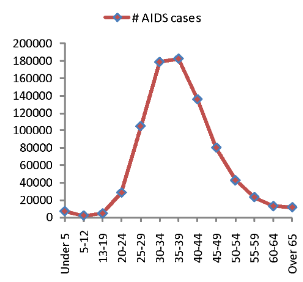
\includegraphics[width=\linewidth]{Pictures/aids-line.png}
        \caption{Line Chart}
        \label{fig:aids-line}
    \end{subfigure}
    \hfill
    \begin{subfigure}[c]{0.45\linewidth}
        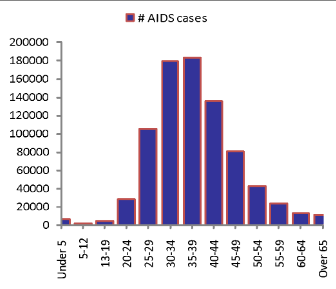
\includegraphics[width=\linewidth]{Pictures/aids-histogram.png}
        \caption{Histogram}
        \label{fig:aids-histogram}
    \end{subfigure}
    \caption{Distribution data: Histogram is a better choice
    if discrete groups}
    \label{fig:aids-distribution}
  \end{figure}
\end{example}

\begin{example}
  \textbf{Seasonality in Sales Data}: Use a line chart to show
  seasonality in sales data or other time series data.

  \begin{figure}[hitb!]
    \centering
    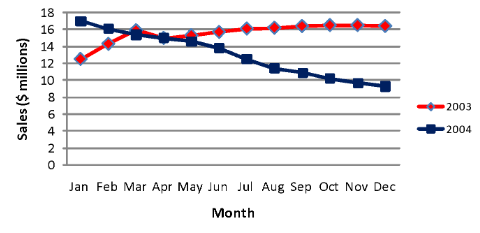
\includegraphics[width=0.8\linewidth]{Pictures/seasonality.png}
    \caption{Seasonality in Sales Data}
    \label{fig:seasonality}
  \end{figure}
\end{example}

\subsection{Chart or Table?}

Sometimes a table is better than a chart.
If the data is small and the audience needs to see the exact values,
then a table is better than a chart.

This is also the case if there is no pattern in the data to be shown.

\subsection{Appropriate Chart Type for Different types of Messages}

We can also use a simple heuristic to choose the right chart type
based on the message that we want to convey.

\begin{table}[htb!]
  \centering
  \begin{tabular}{|c|c|c|}
    \hline
    \textbf{Message} & \textbf{Chart Type} & \textbf{Example} \\
    \hline
    \textbf{Item Comparison} & Bar Chart
    & 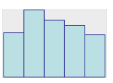
\includegraphics[width=0.1\linewidth]{Pictures/small-bar.png} \\
    \hline
    \textbf{Components of one item} & Pie Chart
    & 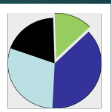
\includegraphics[width=0.1\linewidth]{Pictures/small-pie.png} \\
    \hline
    \textbf{Components of multiple item} & Stacked Bar Chart
    & 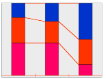
\includegraphics[width=0.1\linewidth]{Pictures/small-stacked-bar.png} \\
    \hline
    \textbf{Distribution} & Histogram
    & 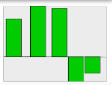
\includegraphics[width=0.1\linewidth]{Pictures/small-histogram.png} \\
    \hline
    \textbf{Relationship} & Scatter Plot
    & 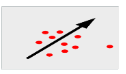
\includegraphics[width=0.1\linewidth]{Pictures/small-scatter.png} \\
    \hline
    \textbf{Location} & Map
    & 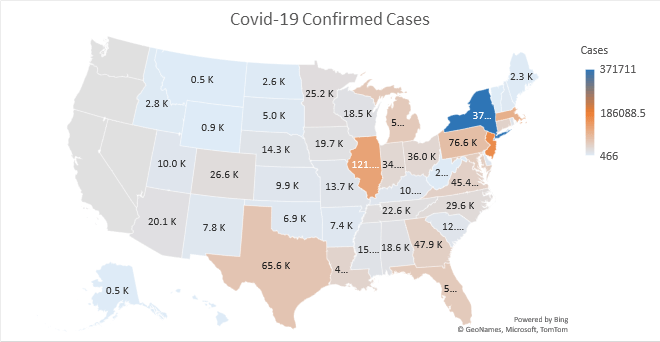
\includegraphics[width=0.1\linewidth]{Pictures/small-map.png} \\
    \hline
    \textbf{Change over Time} & Line Chart
    & 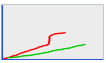
\includegraphics[width=0.1\linewidth]{Pictures/small-line.png} \\
    \hline
    \textbf{Outliers} & Box Plot
    & 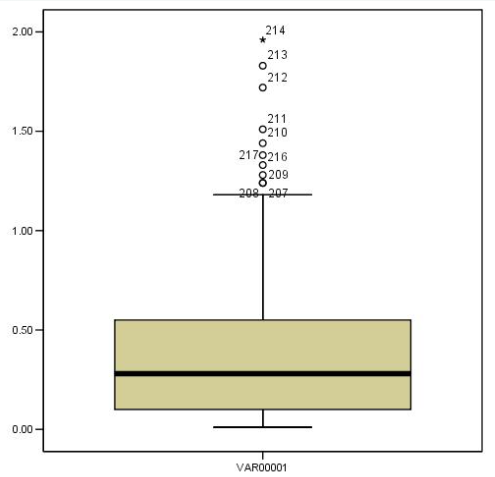
\includegraphics[width=0.1\linewidth]{Pictures/small-box.png} \\
    \hline
  \end{tabular}
  \caption{Appropriate Chart Type for Different types of Messages}
  \label{tab:chart-type}
\end{table}

\subsection{Designing the Visualization}

Designing is a very important step in data visualization.
The design should ensure quick cognitive processing of the visualization.
The design should also be aesthetically pleasing.\\

A few best practices for designing visualizations are:

\begin{itemize}
  \item \textbf{Avoid 3D Charts}:
    3D charts are hard to read and understand.
    They also distort the data by violating the
    \textbf{Area Principle}.
  \item \textbf{Avoid Legends}:
    Legends are hard to read and understand.
    It is better to label the data directly.
  \item \textbf{Maintain High Contrast}:
    The colors used in the visualization should have
    high contrast. This makes the visualization easy to read.
  \item \textbf{Annotate Data to highlight important points}:
    Annotations help the audience understand the visualization.
    They also help the audience focus on the important points.
\end{itemize}

\begin{figure}[hibt!]
  \centering
  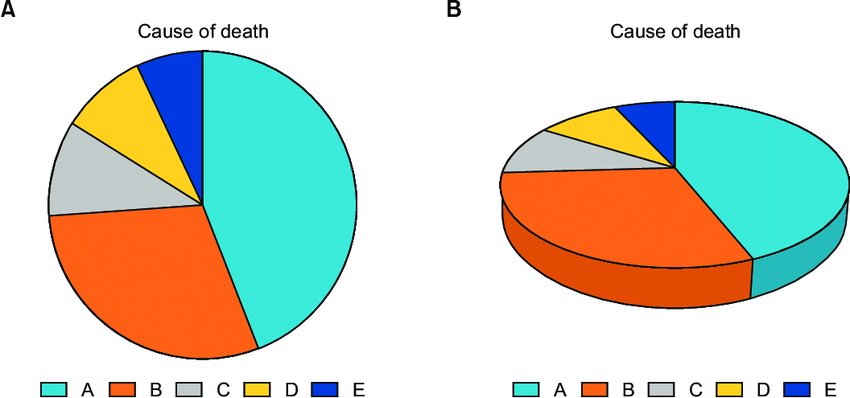
\includegraphics[width=0.8\linewidth]{Pictures/area-principle.png}
  \caption{Area Principle is violated in 3D Charts; avoid them}
  \label{fig:area-principle}
\end{figure}

\begin{figure}[hibt!]
  \centering
  \begin{subfigure}[c]{0.45\linewidth}
      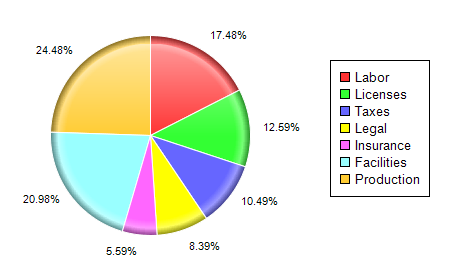
\includegraphics[width=\linewidth]{Pictures/pie-legend.png}
      \caption{Pie Chart with Legend}
      \label{fig:pie-legend}
  \end{subfigure}
  \begin{subfigure}[c]{0.35\linewidth}
      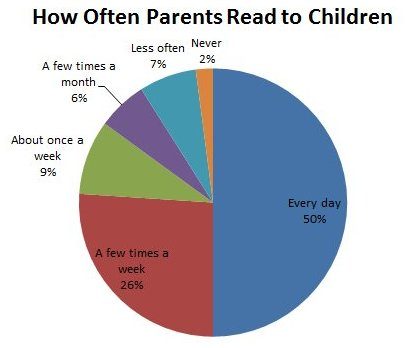
\includegraphics[width=\linewidth]{Pictures/pie-label.jpg}
      \caption{Pie Chart with Labels}
      \label{fig:pie-label}
  \end{subfigure}
  \caption{Pie with Labels is easier to read than Pie with Legend}
  \label{fig:pie-label-over-legend}
\end{figure}

\begin{figure}[hibt!]
  \centering
  \includegraphics[width=0.75\linewidth]{Pictures/pie-vs-bar.png}
  \caption{Bar Charts are better than Pie Charts if
  the number of categories is large}
  \label{fig:pie-vs-bar}
\end{figure}

\section{Visualizing Data in Dashboards}

\begin{definition}[Dashboard]
  A dashboard is a visual display of the most important information
  needed to achieve one or more objectives;
  consolidated and arranged on a single screen, so the information
  can be monitored at a glance.
\end{definition}

\begin{figure}[htb!]
  \centering
  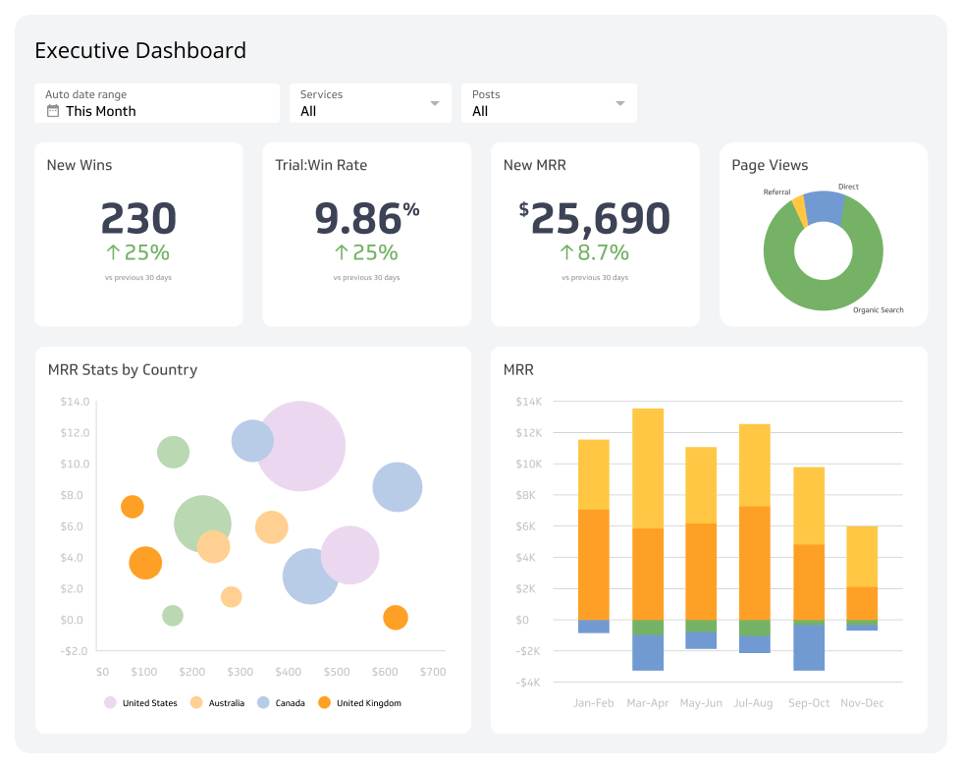
\includegraphics[width=0.7\linewidth]{Pictures/dashboard.png}
  \caption{Example Dashboard}
  \label{fig:dashboard}
\end{figure}


\subsection{Why Dashboards?}

Dashboards connect all kinds of different metrics, data sources, APIs, and
services to help companies extract relevant information from those sources and
display it in user-friendly ways.
Like a car’s dashboard, data dashboards organize and display important
information at a glance to help you understand your company’s most valuable
data and unearth answers to crucial questions.
By connecting dashboards to specific metrics or key performance indicators
(KPIs), you gain vital business intelligence and the ability to dive deep into
specific pieces of information to continually monitor success.

\subsection{Tools}

Dashboard can be designed using multiple applications. Some of them are:

\begin{itemize}
  \item \textbf{Microsoft Excel} or \textbf{Google Sheets}
  \item \textbf{Microsoft Power BI}
  \item \textbf{Tableau}
  \item \textbf{Google Data Studio}
\end{itemize}
Enterprise dashboards are usually designed using Microsoft Power BI or Tableau.
But simple dashboards can be designed using Microsoft Excel or Google Sheets.

\newpage

\section{Exercises}

\begin{question}
When do you choose “charts” for representing data?
  \begin{enumerate}[label=(\alph*)]
    \item To show how data changes over time
    \item Show distribution of data
    \item Show complete data
    \item Show slice of data
\end{enumerate}
\end{question}

\begin{rotanswer}
  (a), (b), (d)
\end{rotanswer}

\begin{question}
  When do you \textbf{not} choose a table to represent data?
  \begin{enumerate}[label=(\alph*)]
    \item Display complete data
    \item Highlight specific item in context of complete data
    \item Show patterns in data
    \item None of the above
\end{enumerate}
\end{question}

\begin{rotanswer}
  (c)
\end{rotanswer}

\begin{question}
 Select which of the following are categorical data?
  \begin{enumerate}[label=(\alph*)]
    \item Your highest level of education
    \item Customer rating for service experience e.g. Poor, Average, Good.
    \item Your age bucket e.g. below 18 year, between 19 and 30 years etc.
    \item Time
    \item Pressure
\end{enumerate}
\end{question}

\begin{rotanswer}
  (a), (b), (c)
\end{rotanswer}

\begin{question}
Q4. Select which of the following are discrete data?
  \begin{enumerate}[label=(\alph*)]
    \item How many siblings do you have?
    \item Weight
    \item Number of houses in your locality
    \item Defects per hour
    \item Pressure
\end{enumerate}
\end{question}

\begin{rotanswer}
  (a), (c), (d)
\end{rotanswer}

\begin{question}
Q5. Select which of the following are continuous data?
  \begin{enumerate}[label=(\alph*)]
    \item Time between two successive failures of an equipment
    \item Volume
    \item Gender
    \item Your favourite cuisines
    \item Density
\end{enumerate}
\end{question}

\begin{rotanswer}
  (a), (b), (e)
\end{rotanswer}

\begin{question}
  Q6. Which chart is used for what type of data?
  \begin{multicols}{2}
    \begin{enumerate}[label=(\alph*)]
      \item Box Plot
      \item Line Chart
      \item Bar Chart
      \item Column / Stacked Column Chart
      \item Histogram
      \item Scatter Plot
      \item Pie Chart
    \end{enumerate}
    \columnbreak
    \begin{enumerate}[label=(\roman*)]
      \item One item proportional to totals
      \item Multiple items components
      \item Comparison between items
      \item Trend over time
      \item Frequency of items
      \item Outlier identification
      \item Correlation representation
    \end{enumerate}
  \end{multicols}
\end{question}

\begin{rotanswer}
  The matching is as follows:
  \begin{enumerate}[label=(\alph*)]
    \item (vi)
    \item (iv)
    \item (iii)
    \item (ii)
    \item (v)
    \item (vii)
    \item (i)
  \end{enumerate}
\end{rotanswer}


\newpage

\begin{remark}
Table-1 below provides the country wise sales of items A, B, C, D, and E.
Then for the messages in questions 7, 8, and 9, choose the
appropriate best representation from the given options
\end{remark}

\begin{figure}[hitb!]
  \centering
  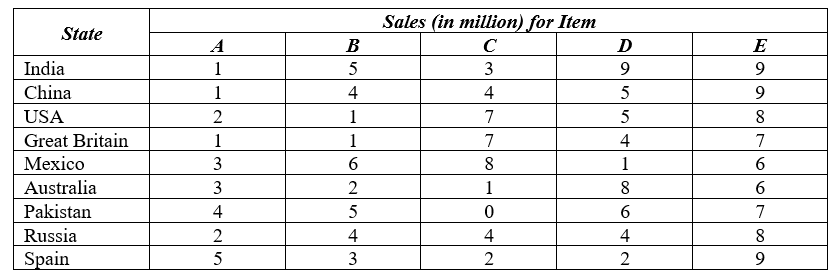
\includegraphics[width=0.7\linewidth]{Pictures/PA1b.png}
  \caption{PA 1 Table}
  \label{fig:pa1-table}
\end{figure}

\begin{question}
Message to convey: “Country with the highest sales for each item”
\end{question}
\begin{figure}[hitb!]
  \centering
  \begin{subfigure}[c]{0.75\linewidth}
    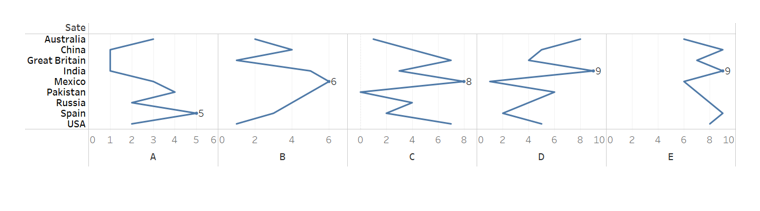
\includegraphics[width=\linewidth]{Pictures/op1.png}
    \caption{Option 1}
    \label{fig:pa1-op1}
  \end{subfigure}
  \hfill
  \begin{subfigure}[c]{0.35\linewidth}
    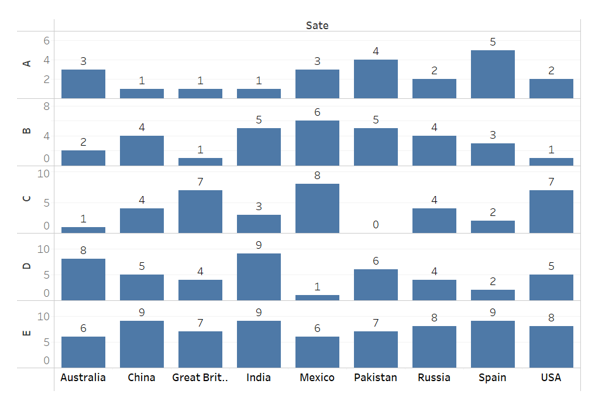
\includegraphics[width=\linewidth]{Pictures/op2.png}
    \caption{Option 2}
    \label{fig:pa1-op2}
  \end{subfigure}
  \begin{subfigure}[c]{0.35\linewidth}
    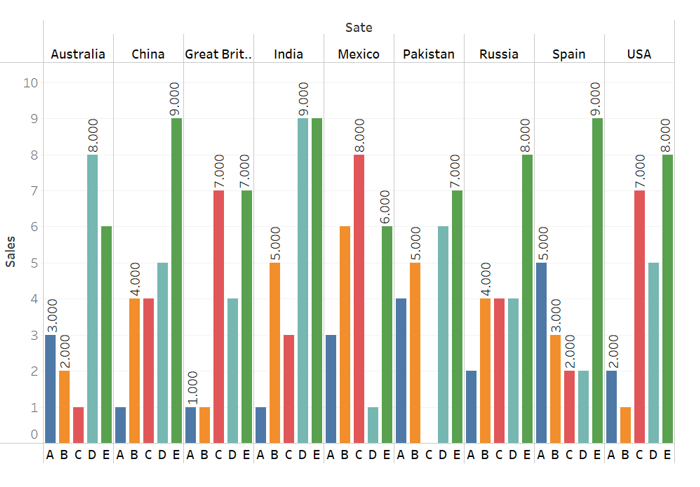
\includegraphics[width=\linewidth]{Pictures/op3.png}
    \caption{Option 3}
    \label{fig:pa1-op3}
  \end{subfigure}
  \hfill
  \begin{subfigure}[c]{0.35\linewidth}
    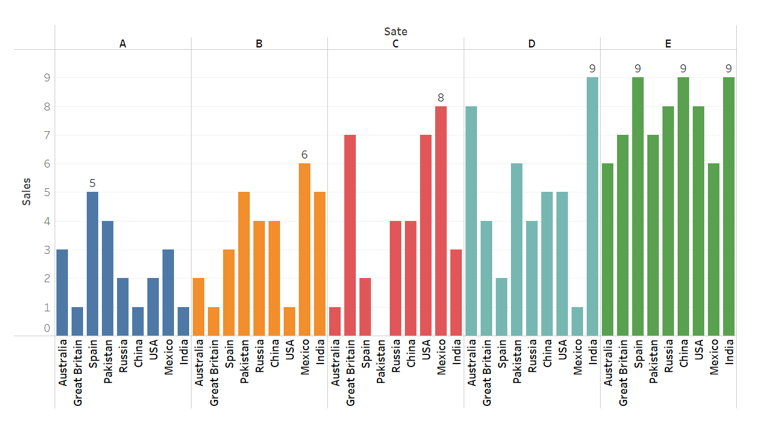
\includegraphics[width=\linewidth]{Pictures/op4.png}
    \caption{Option 4}
    \label{fig:pa1-op4}
  \end{subfigure}
  \caption{Options for Q7}
  \label{fig:pa1-op}
\end{figure}

\begin{rotanswer}
  (d)
\end{rotanswer}

\begin{question}
Message to convey: “Country with the highest sales across all items”
\end{question}

\begin{figure}[hitb!]
  \centering
  \begin{subfigure}[c]{0.45\linewidth}
    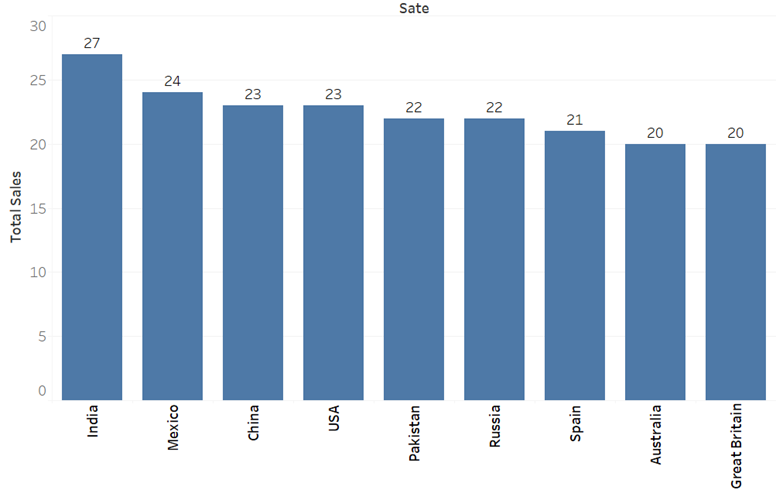
\includegraphics[width=\linewidth]{Pictures/paq8-1.png}
    \caption{Option 1}
    \label{fig:pa1.8-op1}
  \end{subfigure}
  \hfill
  \begin{subfigure}[c]{0.45\linewidth}
    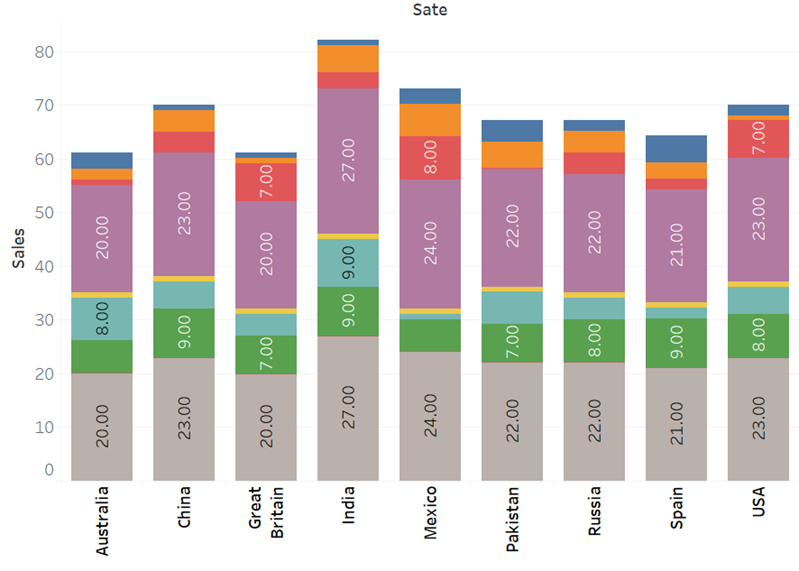
\includegraphics[width=\linewidth]{Pictures/paq8-2.png}
    \caption{Option 2}
    \label{fig:pa1.8-op2}
  \end{subfigure}
  \begin{subfigure}[c]{0.45\linewidth}
    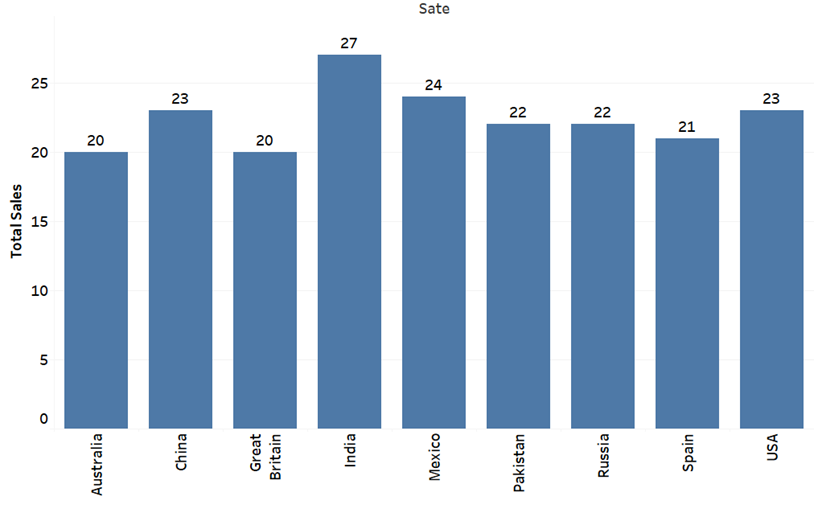
\includegraphics[width=\linewidth]{Pictures/paq8-3.png}
    \caption{Option 3}
    \label{fig:pa1.8-op3}
  \end{subfigure}
  \hfill
  \begin{subfigure}[c]{0.45\linewidth}
    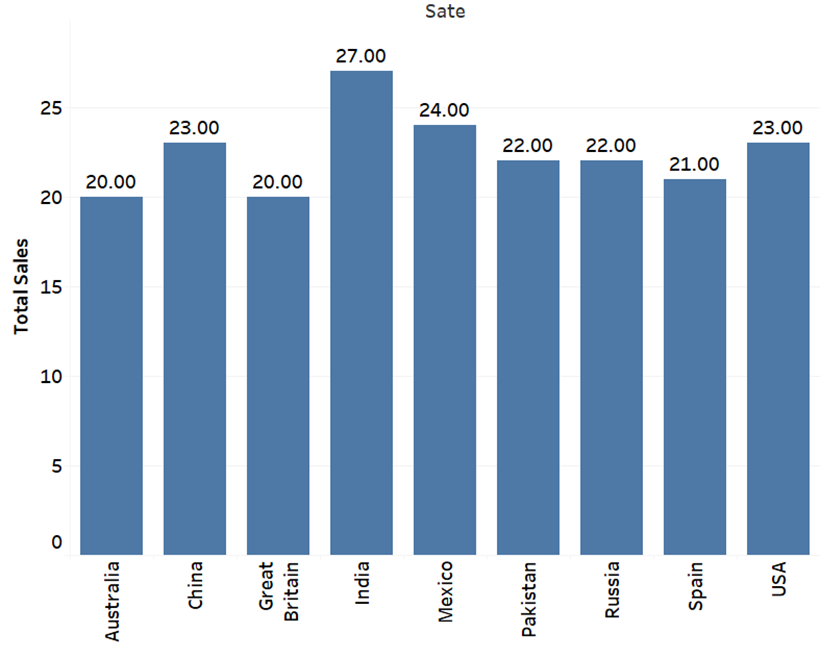
\includegraphics[width=\linewidth]{Pictures/paq8-4.png}
    \caption{Option 4}
    \label{fig:pa1.8-op4}
  \end{subfigure}
  \caption{Options for Q8}
  \label{fig:pa1.8-op}
\end{figure}

\begin{rotanswer}
  (a)
\end{rotanswer}

\newpage

\begin{question}
Message to convey: “Across all items, the country wise proportion of item-A being sold”
\end{question}

\begin{figure}[hitb!]
  \centering
  \begin{subfigure}[c]{0.45\linewidth}
    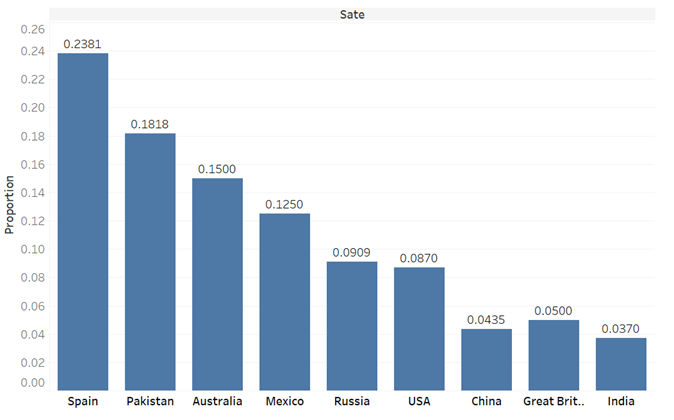
\includegraphics[width=\linewidth]{Pictures/paq9-1.png}
    \caption{Option 1}
    \label{fig:pa1.9-op1}
  \end{subfigure}
  \hfill
  \begin{subfigure}[c]{0.45\linewidth}
    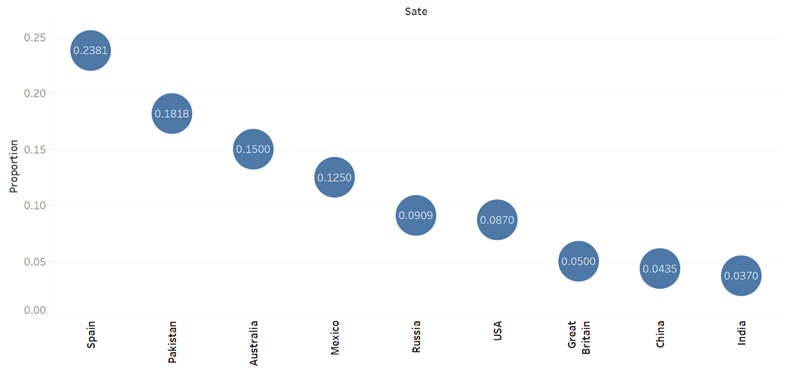
\includegraphics[width=\linewidth]{Pictures/paq9-2.png}
    \caption{Option 2}
    \label{fig:pa1.9-op2}
  \end{subfigure}
  \begin{subfigure}[c]{0.45\linewidth}
    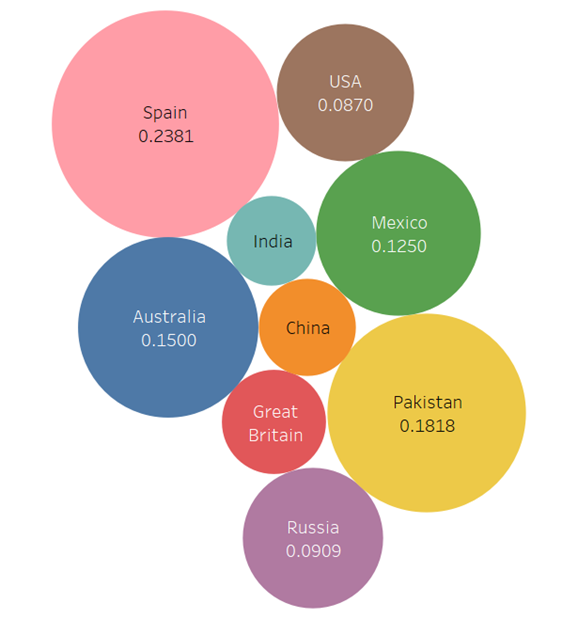
\includegraphics[width=\linewidth]{Pictures/paq9-3.png}
    \caption{Option 3}
    \label{fig:pa1.9-op3}
  \end{subfigure}
  \hfill
  \begin{subfigure}[c]{0.45\linewidth}
    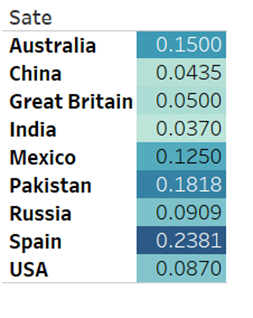
\includegraphics[width=\linewidth]{Pictures/paq9-4.png}
    \caption{Option 4}
    \label{fig:pa1.9-op4}
  \end{subfigure}
  \caption{Options for Q9}
  \label{fig:pa1.9-op}
\end{figure}

\begin{rotanswer}
  (a), (b), (d)
\end{rotanswer}

\end{document}
